\section{Terrain}

The terrain is the main topic of this project so let's start to introduce the different components.

\subsection{Cell}
\noindent
The main part of the terrain is a cell, a cell is basically a square whose sides have a fixed and equal size and number of vertices. As you can imagine, a cell at first is just a plane, as large as the multiplication \textbf {Dimension x Dimension} and with \textbf {Vertices x Vertices} number of vertices. Creating a plane is not a difficult task, so I didn't load a model but I generated it manually. First, I created the different vertices and stored them in a vector, then I generated the different indices to create the triangles of the mesh.

\begin{figure}[hbt!]
	\centering
	\subfloat[\centering Plane.]{{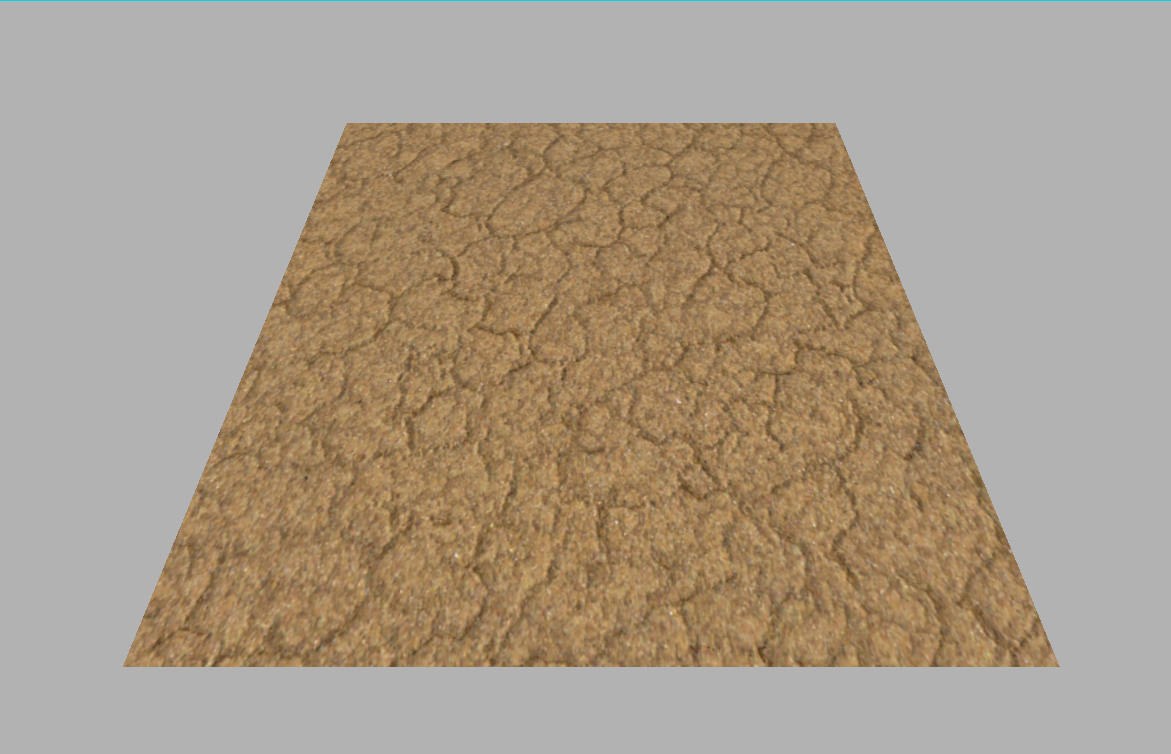
\includegraphics[width=6.3cm]{images/terrain1Normal.png}}}%
	\qquad
	\subfloat[\centering Vertices, indices and faces.]{{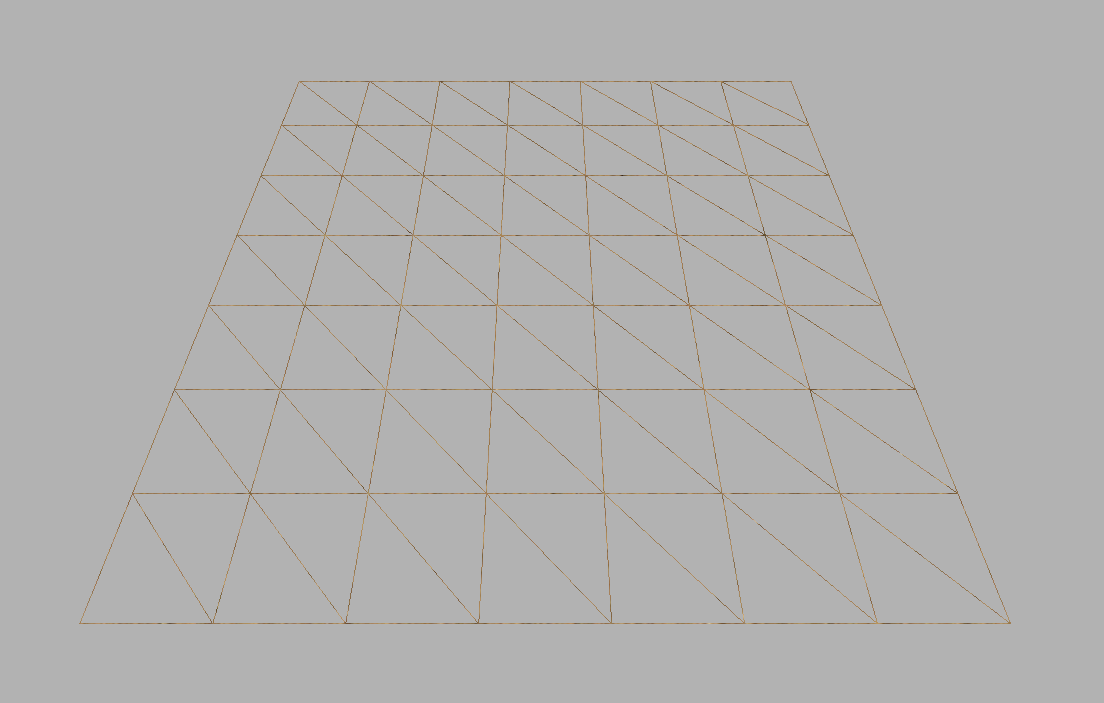
\includegraphics[width=6.3cm]{images/terrain1Vertices.png} }}%
	\caption{}
\end{figure}

\noindent
Obviously I didn't want flat ground, so I had to introduce some noises. For this task I relied on an existing library called \textbf{FastNoiseLite} which implemented different types of noise function. You can set various parameters, such as the type of noise, the seed and the frequency. In this specific case I choose a Perlin noise type, a random seed and a noise frequency of 0.008. By changing these parameters you can get different terrains.
In addition, the maximum height of the terrain must also be specified. Then, at the time of creation, each vertex generates a noise that will be multiplied by the maximum height.

\newpage
\begin{figure}[hbt!]
	\centering
	\subfloat[\centering Front plane.]{{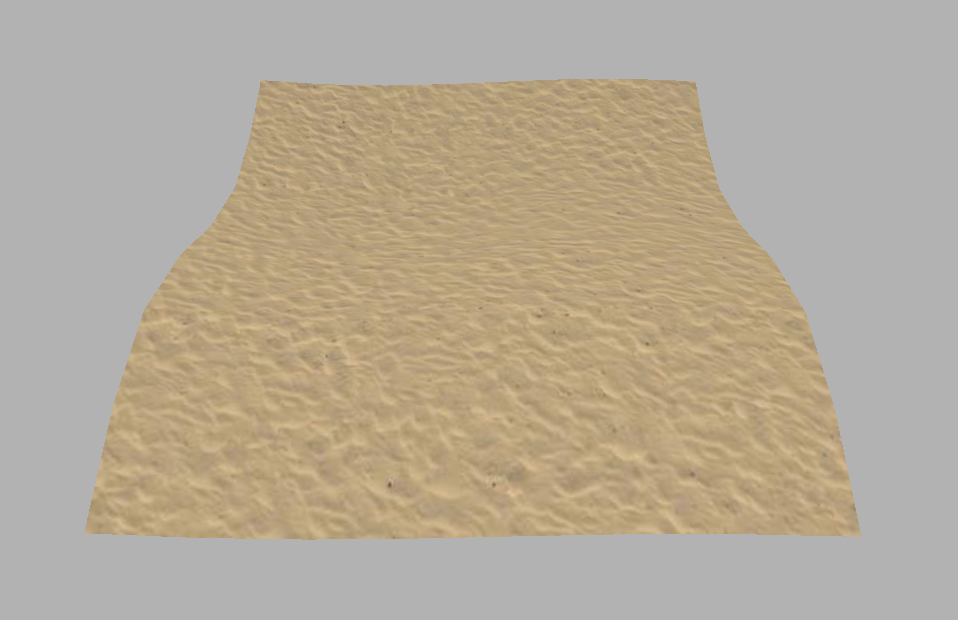
\includegraphics[width=6.3cm]{images/terrain2Front.png}}}%
	\qquad
	\subfloat[\centering Side plane.]{{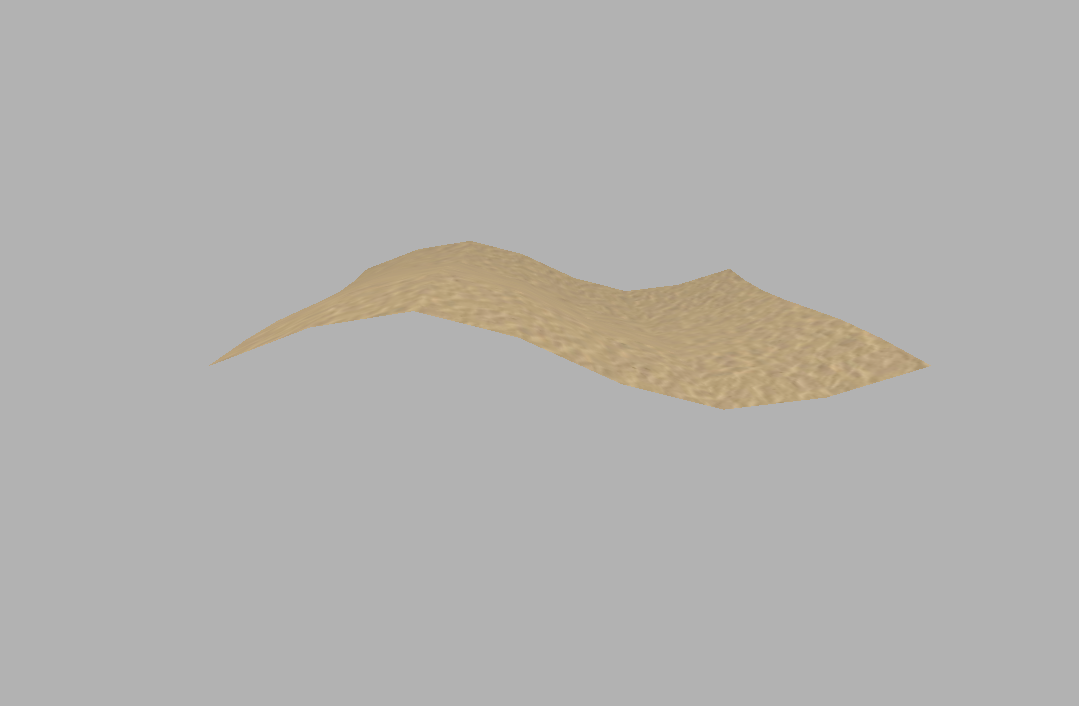
\includegraphics[width=6.3cm]{images/terrain2Side.png} }}%
	\caption{}
\end{figure}

\noindent
For any other information about a cell, you can check the \textbf{terrain.h} file.

\subsection{Terrain}

To create a large terrain, I put several cells together, specifically I create a square of cells. Basically I just have to choose the number of cells per row/column and put them close together. What I get now is something pretty awful, because there is no correlation between the height of the adjacent cells but it is totally random.

\smallbreak

\begin{figure}[hbt!]
	\centering
	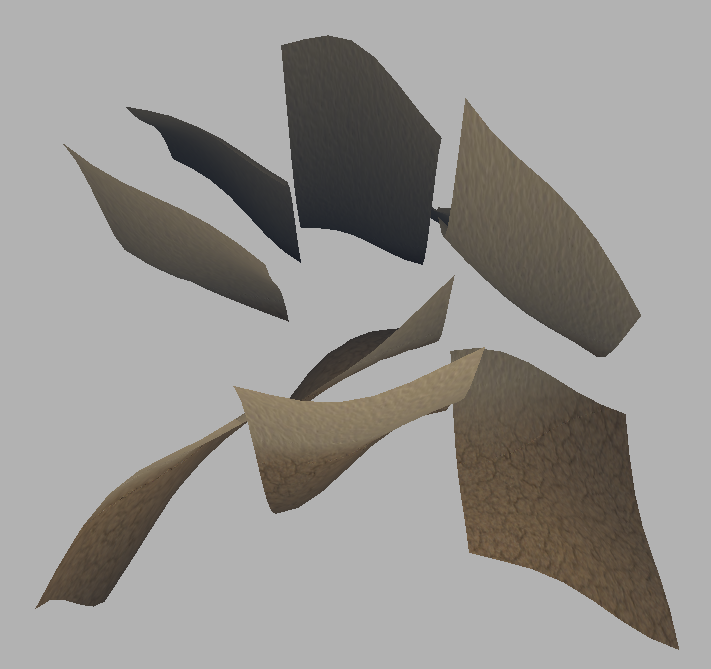
\includegraphics[width= 0.55
	\textwidth]{images/terrain3.png}
	\caption{This image represents 9 cells (3 per row) with random heights.}
\end{figure} 

\newpage

\subsection{Blending}
The simple solution is to use a blending function between two adjacent cells.
we can summarize this process in three parts.

\subsubsection{First Part}

Since I am doing this process on adjacent cells, they obviously need to reach the same height on the common side. The simplest way to accomplish this, is to use a simple lerp function that averages the heights of two common side vertices and assign it to them.

\begin{figure}[hbt!]
	\centering
	\subfloat[\centering Before.]{{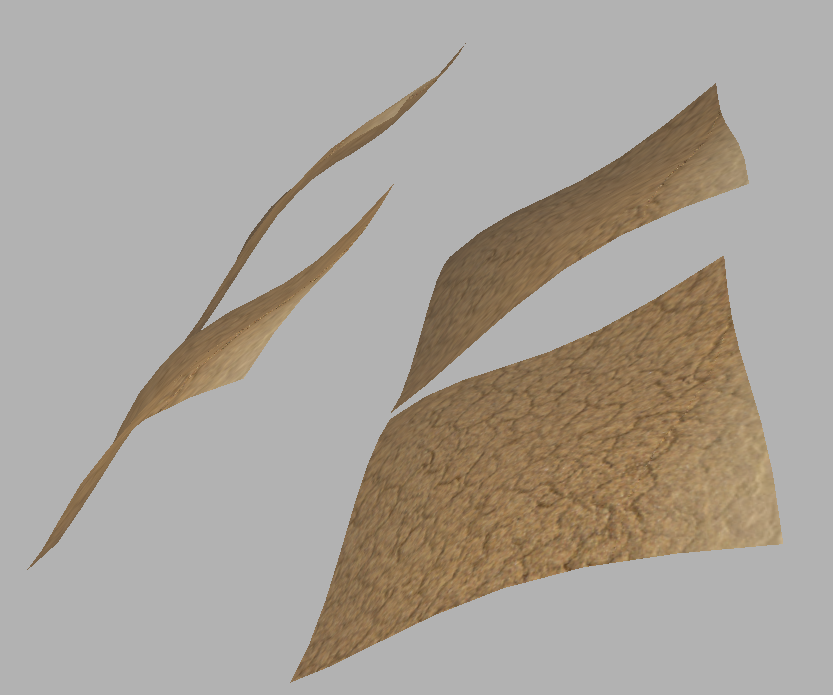
\includegraphics[width=6.3cm]{images/terrain4Before.png}}}%
	\qquad
	\subfloat[\centering After.]{{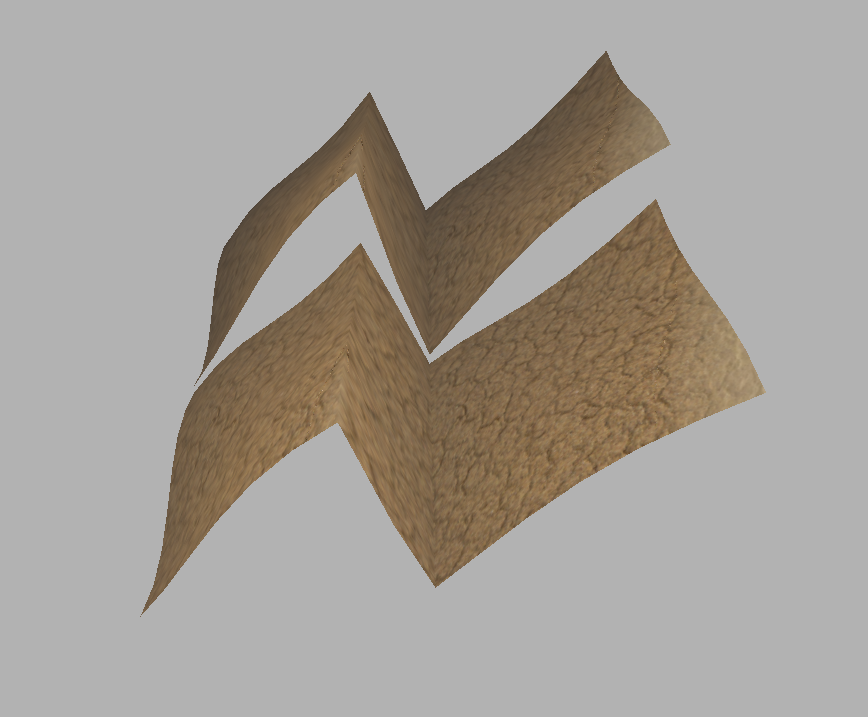
\includegraphics[width=6.3cm]{images/terrain4After.png} }}%
	\caption{}
\end{figure}

\subsubsection{Second and third part}

The second and third steps are actually the same, the only thing that changes is the cell that is used. In particular, it is necessary to propagate the height update obtained on the "hinge" side. We use again a lerp function but this time it's weighted based on the distance from the melt side. It works like this:

	\begin{itemize}
		
		\item I apply the blending from the melt side to the opposite side.
		\item I only change the value of the vertices farther from the "zipper" side. (Otherwise, the two cells will not be connected anymore).
		\item The blending is weighted, the greater the distance between the vertex and the "hinge" and the less propagation will affect the vertices. The most important thing is that the opposite side will not be affected by the blending as it is very important for connecting more than two cells.
			
	\end{itemize}

\noindent
As it is not very easy to explain the process, I have created the image below which I hope will make the process clearer for you. I also write the formula (although it's not that important) where I calculate the weight of the lerp function based on which vertex I am in at the moment (the \textbf{i} variable is a counter in the for loop). I also write the blend value with four vertices for each row / column in correspondence of each column. As you can see from the example, the first red vertex mixes 0.4 of its height with 0.6 of the new one, in fact it is closer to the hinge, so the blending is greater. Instead the second red vertex, since it is on the opposite side, will not be affected and its value will be the same.

\begin{figure}[hbt!]
	\centering
	\vspace*{\fill}

	\noindent\makebox[\textwidth]{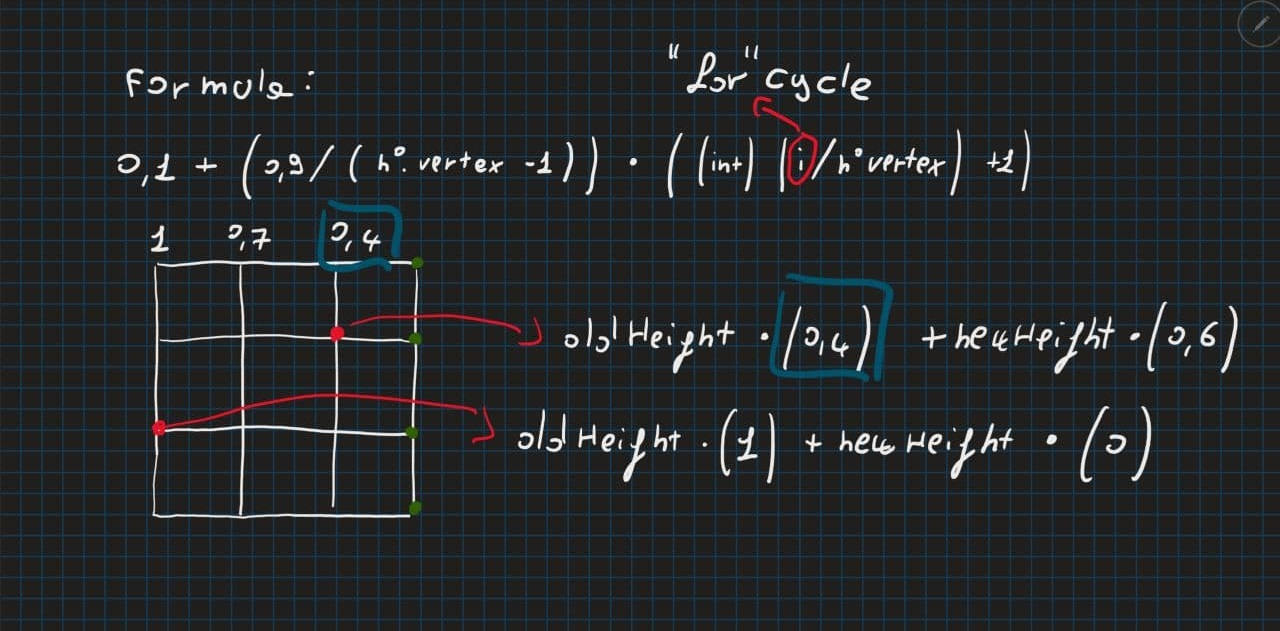
\includegraphics[width=1.4\textwidth,height=0.5\textheight]{images/report1.jpg}}%

	\caption{Visual explanation of the second/third part of the blending.}
\end{figure} 

\newpage

\noindent
So we first apply this propagation to one of the two cell and then we do it for the other one (which why the second part and the third part are the same).

\begin{figure}[hbt!]
	\centering
	\subfloat[\centering Second part.]{{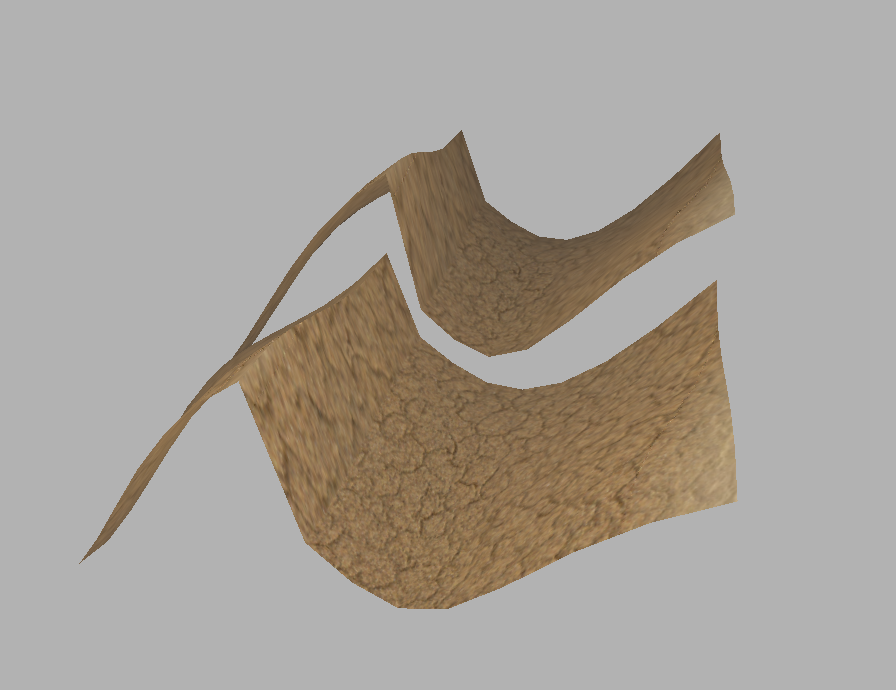
\includegraphics[width=6.3cm]{images/terrain5SecondPart.png}}}%
	\qquad
	\subfloat[\centering Third part.]{{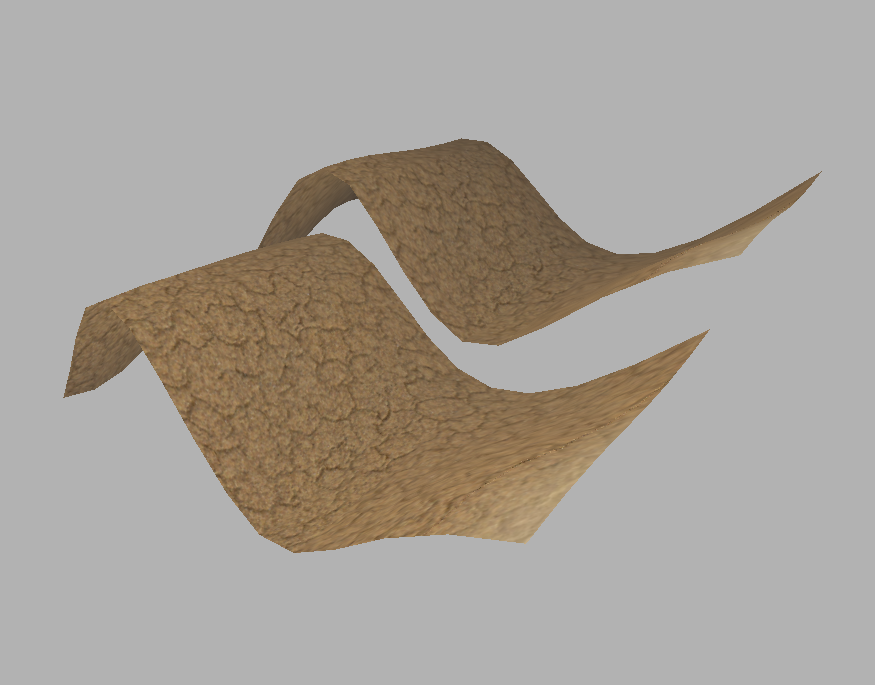
\includegraphics[width=6.3cm]{images/terrain5ThirdPart.png} }}%
	\caption{}
	\label{fig::thirdTerrain}
\end{figure}

\subsubsection{Extra details}
I need to explain two more things. The first is why I want to keep the opposite side unaffected by propagation. Mostly in normal terrain, there will be another cell attached to the opposite side where I have probably already applied the blending process. So I don't have to touch the hinge, otherwise the two cells will separate and I'll have to repeat the process for a potentially infinite number of times.

\begin{figure}[hbt!]
	\centering
	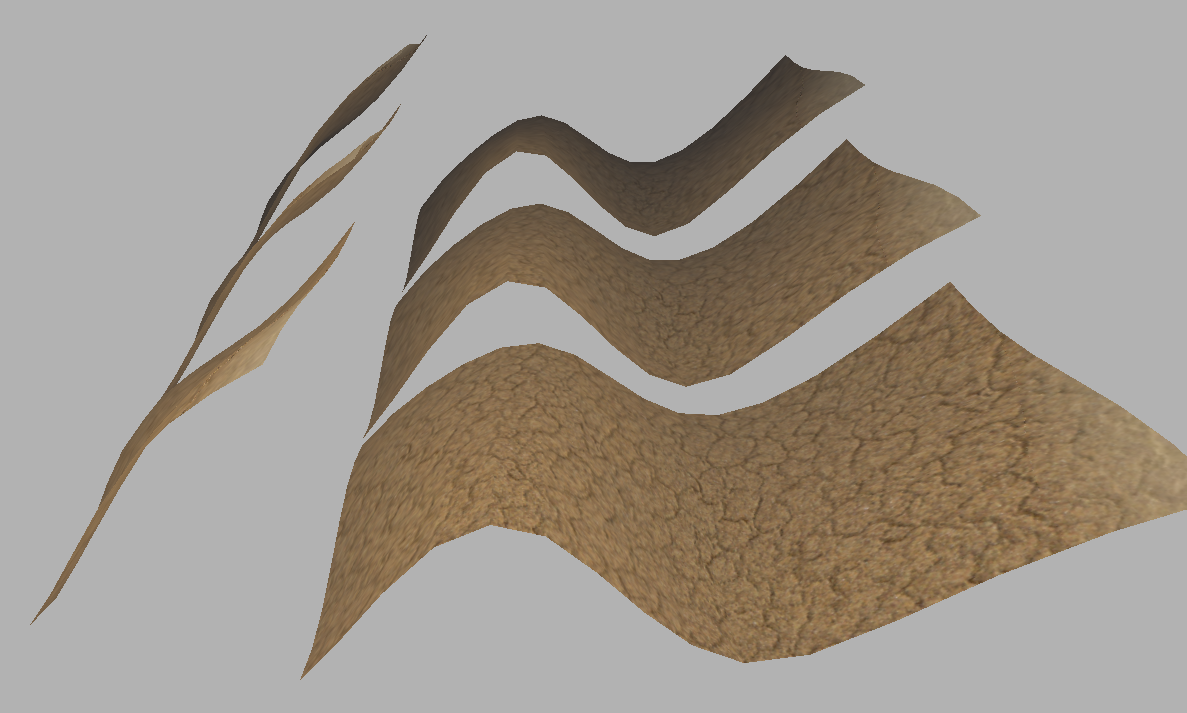
\includegraphics[width= 0.60
	\textwidth]{images/terrain6.png}
	\caption{Before the blending of the left terrain.}
\end{figure} 

\newpage

\begin{figure}[hbt!]
	\centering
	\subfloat[\centering Good blending.]{{\includegraphics[width=6.3cm]{images/terrain6Good.png}}}%
	\qquad
	\subfloat[\centering Bad blending]{{\includegraphics[width=6.3cm]{images/terrain6Bad.png} }}%
	\caption{}
\end{figure}

\noindent
The second thing is that I also have to interpolate the first cell with the last for each row / column. This is because my terrain will be infinite, so if I move a row / column of cells to the opposite side I need them to match the cell in that part. (Explanation of the moving terrain in the \ref{sub::infinteTerrain} section).

\begin{figure}[hbt!]
	\centering
	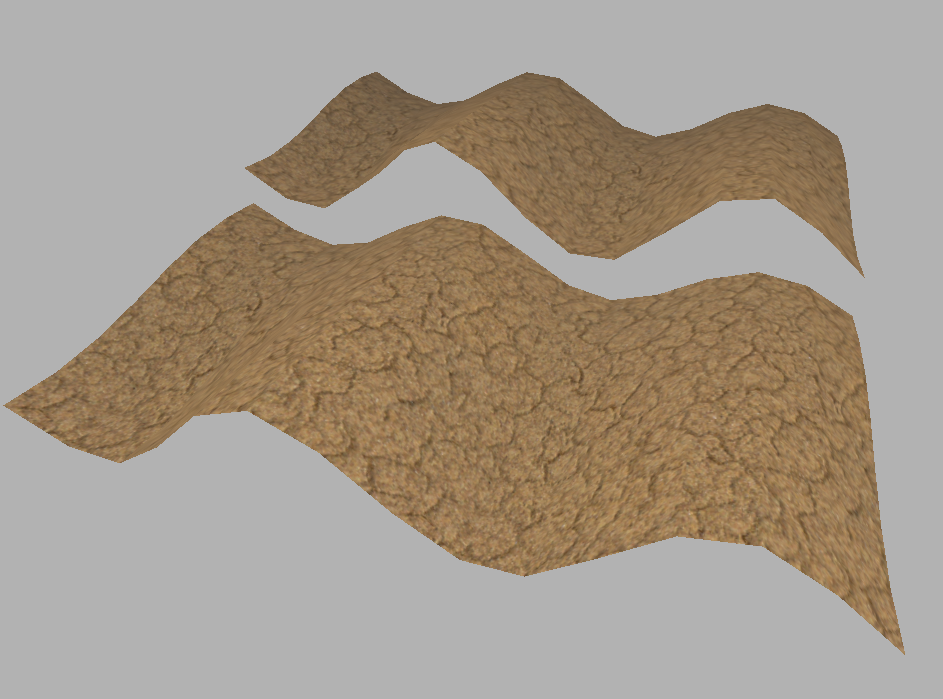
\includegraphics[width= 0.75
	\textwidth]{images/terrain7.png}
	\caption{Final blending between two cells. (Compare it with figure \ref{fig::thirdTerrain}b)}
\end{figure} 

\subsection{Final blending}
I have now got a blend between two cells horizontally, but of course I need it vertically as well. The process is perfectly the same, the only thing to watch out for is not to mix the two interpolations and, before starting the second, you must wait the end of the first.

\begin{figure}[hbt!]
	\centering
	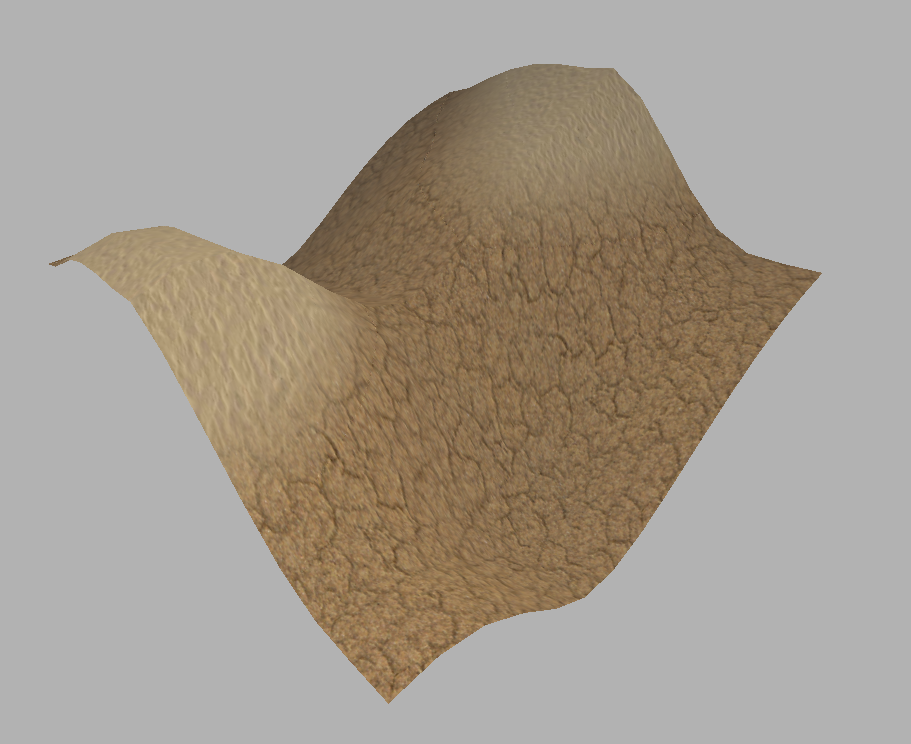
\includegraphics[width= 1
	\textwidth]{images/terrain8.png}
	\caption{Example of horizontal and vertical blending between four cells. (The seed of the cells is different from the one used in the previous example).}
\end{figure} 


\subsection{Infinite terrain}
\label{sub::infinteTerrain}
I want my terrain to move with me, so that it gives the illusion of being infinite. As I said before, our terrain is made up of a fixed number of cells in each row / column so I need to figure out when is the right time to move a cell / column. To explain it, Let's see the image below.

\begin{figure}[hbt!]
	\centering
	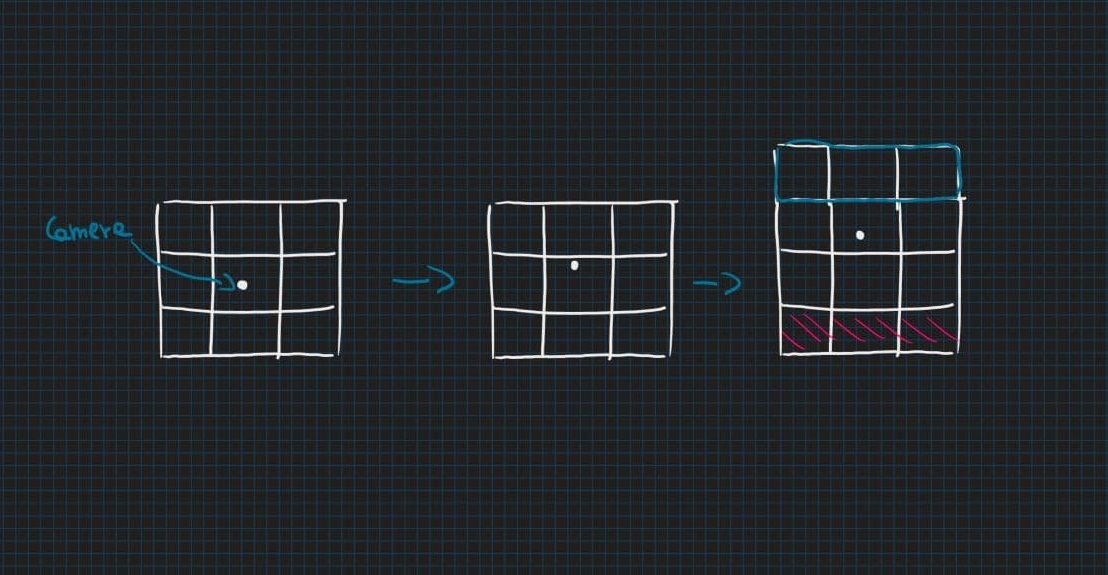
\includegraphics[width= 1
	\textwidth]{images/infiniteTerrainSchema.jpg}
	\caption{Infinite terrain moving schema.}
\end{figure} 

\noindent
Basically to move a row or a column, I check when I overlap another cell and based on the side that I overlapped, I move a column or row on the opposite side. In the above case I am moving forward, so when I reached the end of the middle cell I move the last row to the first position. This is why I need to blend the last row / column as well, so they continue to match perfectly.
In practice what I have to do is simply memorize the indices of the first cell of the last column and row (to get the first I just add the index of a column / row and apply the module operator) so that I can change it to real time and I always know which cells to move.
Obviously the position of the camera is in the central cell. (To keep things simple, I assumed that each row and column had an odd number of cells, so there is always a unique center cell.)

\subsection{Calculate the terrain normals.}
To calculate the normal of a particular vertex, I used a simple method called the "finite difference method" which allowed me to calculate the components of the difference (x, y, z) in a very simple way. Let's start with the x component. I calculated the height near the selected vertex shifting the position in the four direction by a small amount. I first computed the left and right heights, then I subtracted the left one with the right one and obtained the x component. For the z component I do the same but instead of left and right I used the bottom and the top. Finally I set the y component to 2.0. I leave below the simple formula.

\begin{equation}
	normal = vec3(\textcolor{red}{heightLeft} - \textcolor{cyan}{heightRight}, 2.0, \textcolor{magenta}{heightDown} - \textcolor{green}{heightUp})		
\end{equation}

\begin{figure}[hbt!]
	\centering
	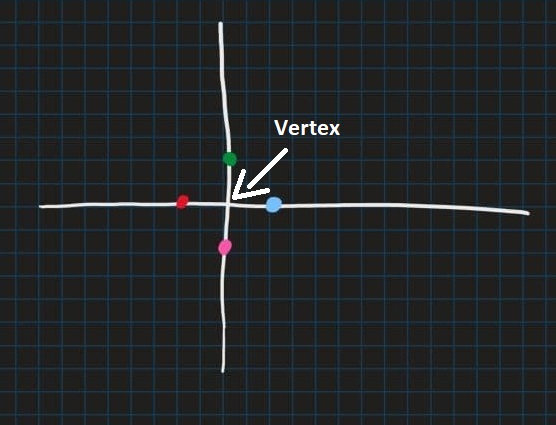
\includegraphics[width= 1
	\textwidth]{images/normalSchema.jpg}
	\caption{Color of the heights considered to calculate the normal in the central vertex.}
\end{figure} 

\noindent
After calculated the normal vector, I normalized it to create a versor.

\subsection{Terrain shader}

\subsubsection{Lambertian light}
Inside the shader there is implemented a simple light model, the Lambertian one. Since it is very simple (the aim was only to check if normals were working, not to create a complex light model) and it isn't different from the one implemented in class, I don't give any others details.

\begin{figure}[hbt!]
	\centering
	\subfloat[\centering No light.]{{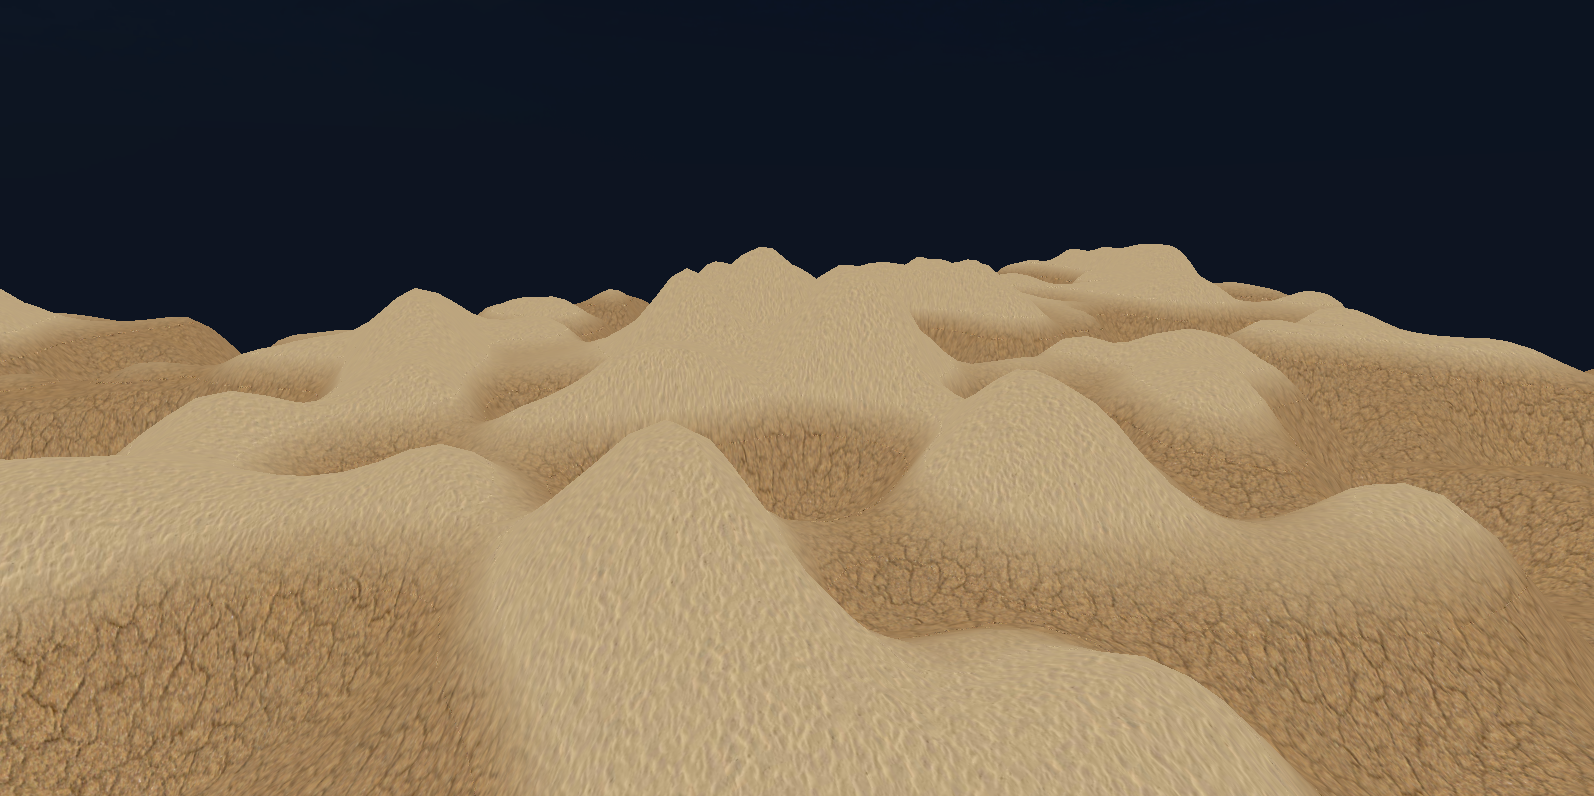
\includegraphics[width=6.3cm]{images/lightTerrainBefore.png}}}%
	\qquad
	\subfloat[\centering Lambertian model.]{{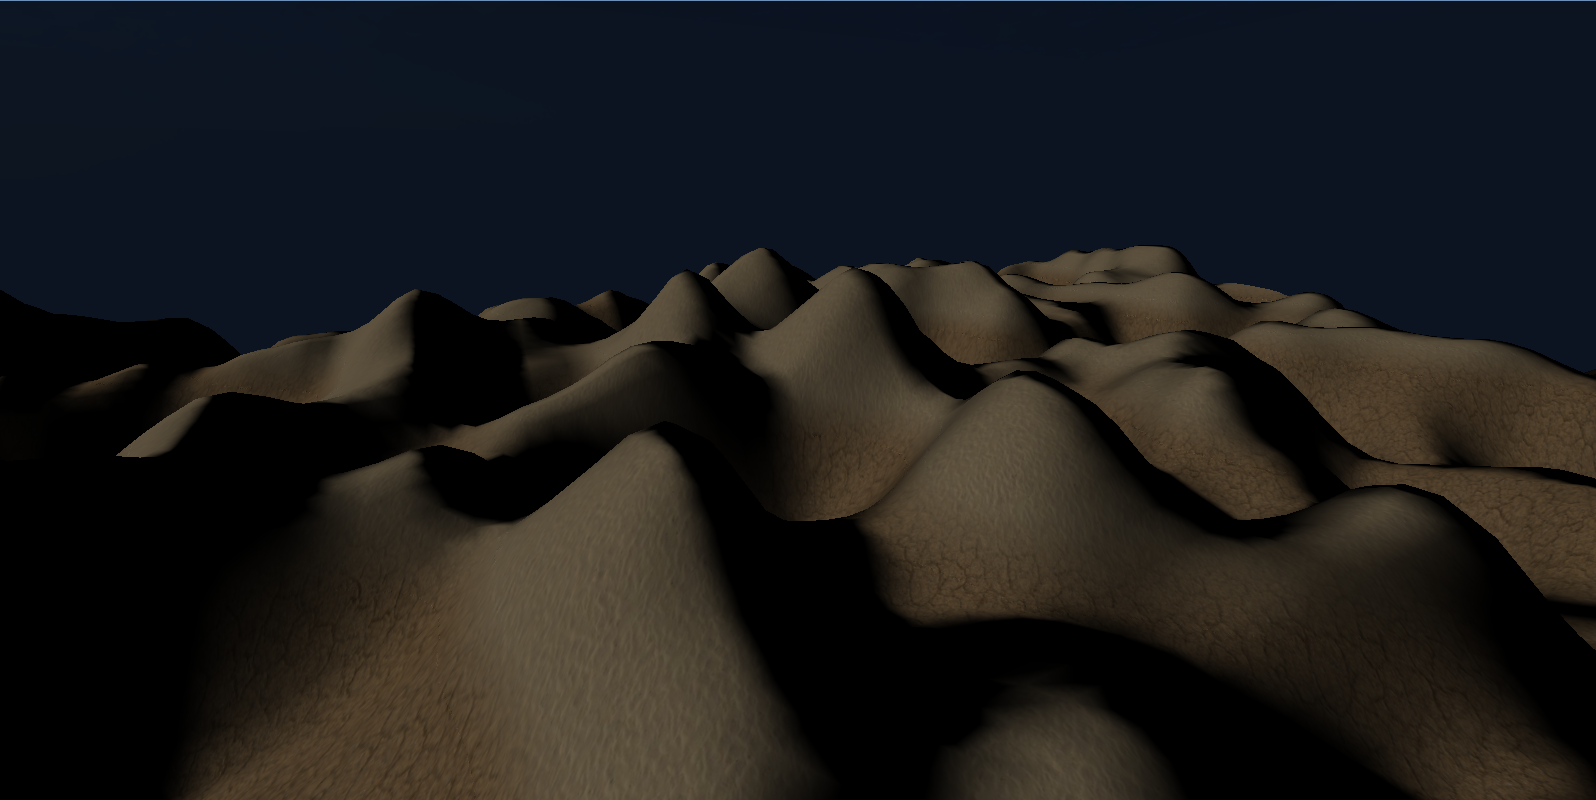
\includegraphics[width=6.3cm]{images/lightTerrainAfter.png} }}%
	\caption{}
\end{figure}

\subsubsection{Multi-texturing}
Instead of assigning a single texture, I used a texture for vertices below a certain height (e.g. up to height < 15), then I used another texture for vertices above another height (e.g. for height > 115). For the central vertices I interpolated the two textures based on the height value.

\begin{figure}[hbt!]
	\centering
	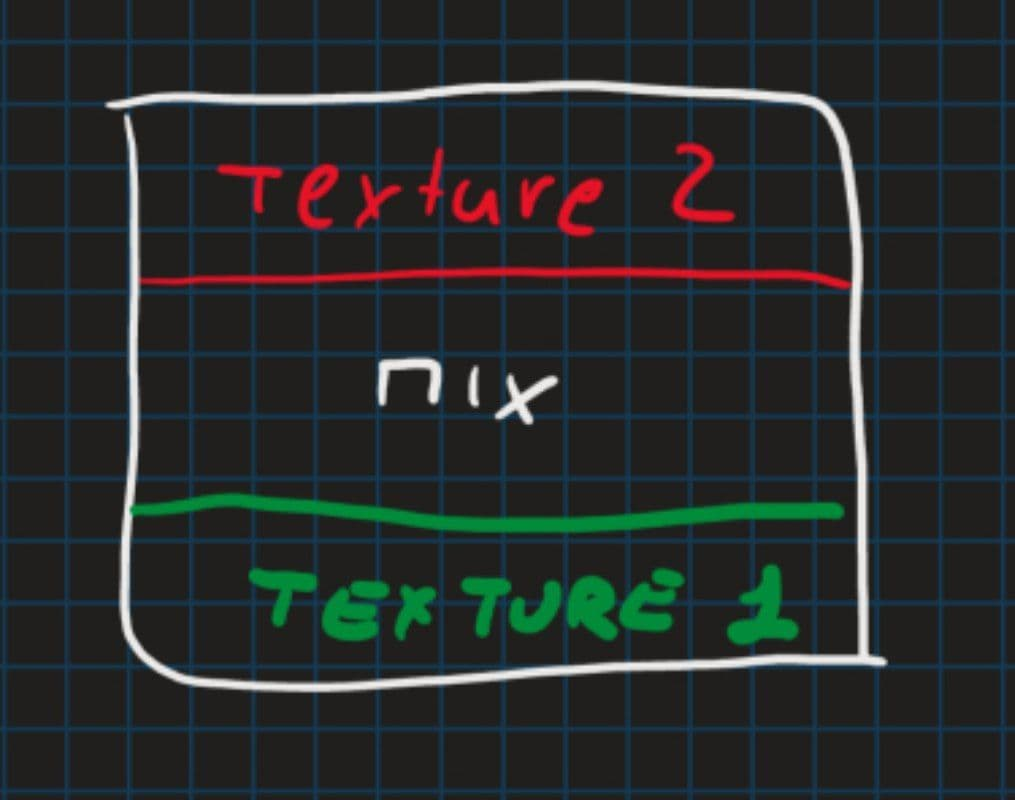
\includegraphics[width= 0.45
	\textwidth]{images/textureSchema.jpg}
	\caption{Multi-texturing schema.}
\end{figure} 

\newpage

\begin{figure}[hbt!]
	\centering
	\subfloat[\centering Terrain one texture.]{{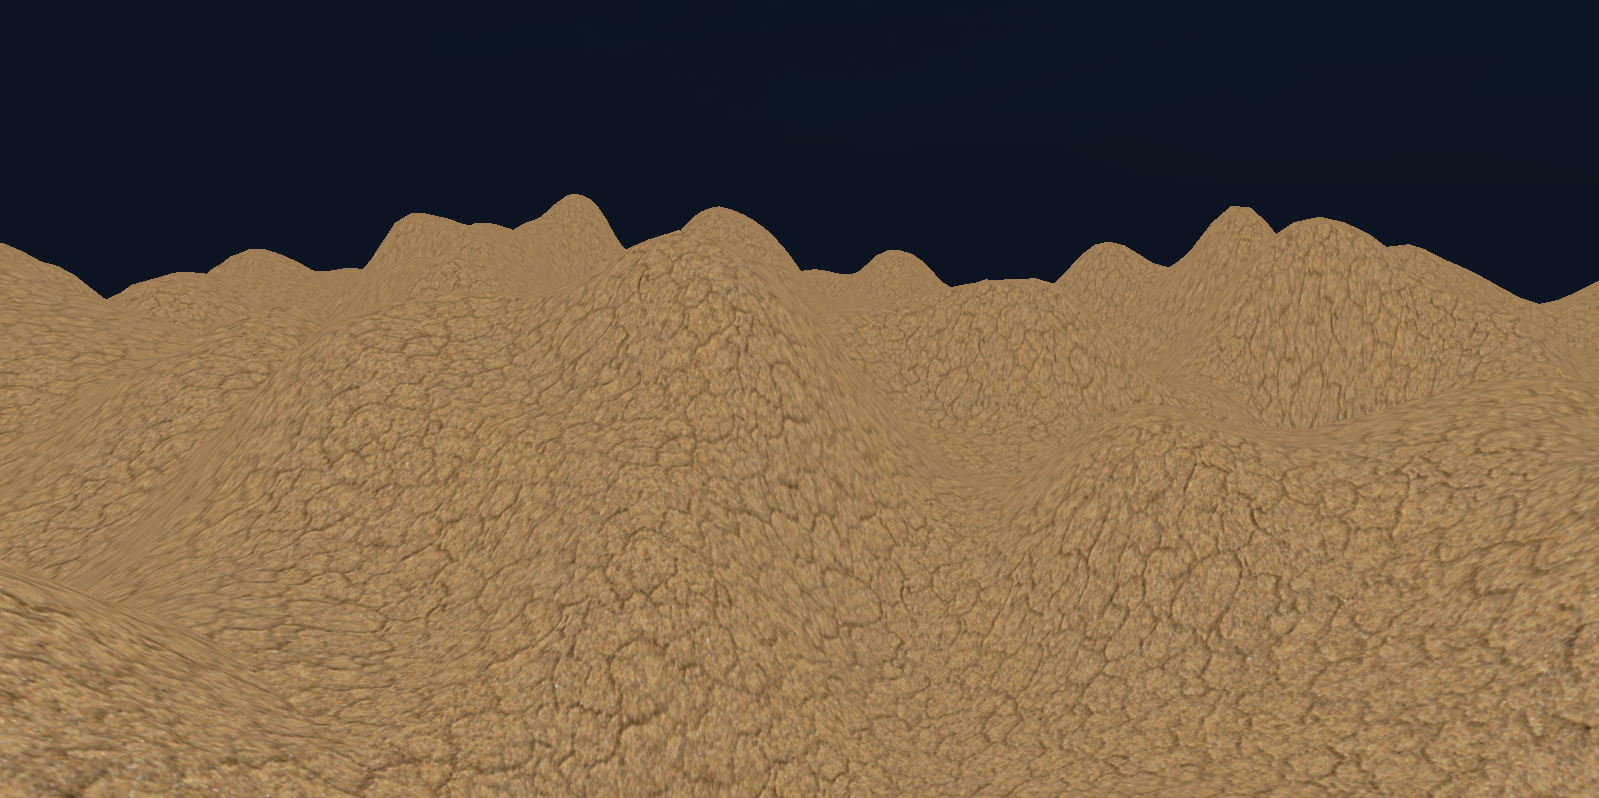
\includegraphics[width=6.3cm]{images/terrain1Texture.png}}}%
	\qquad
	\subfloat[\centering Terrain two textures.]{{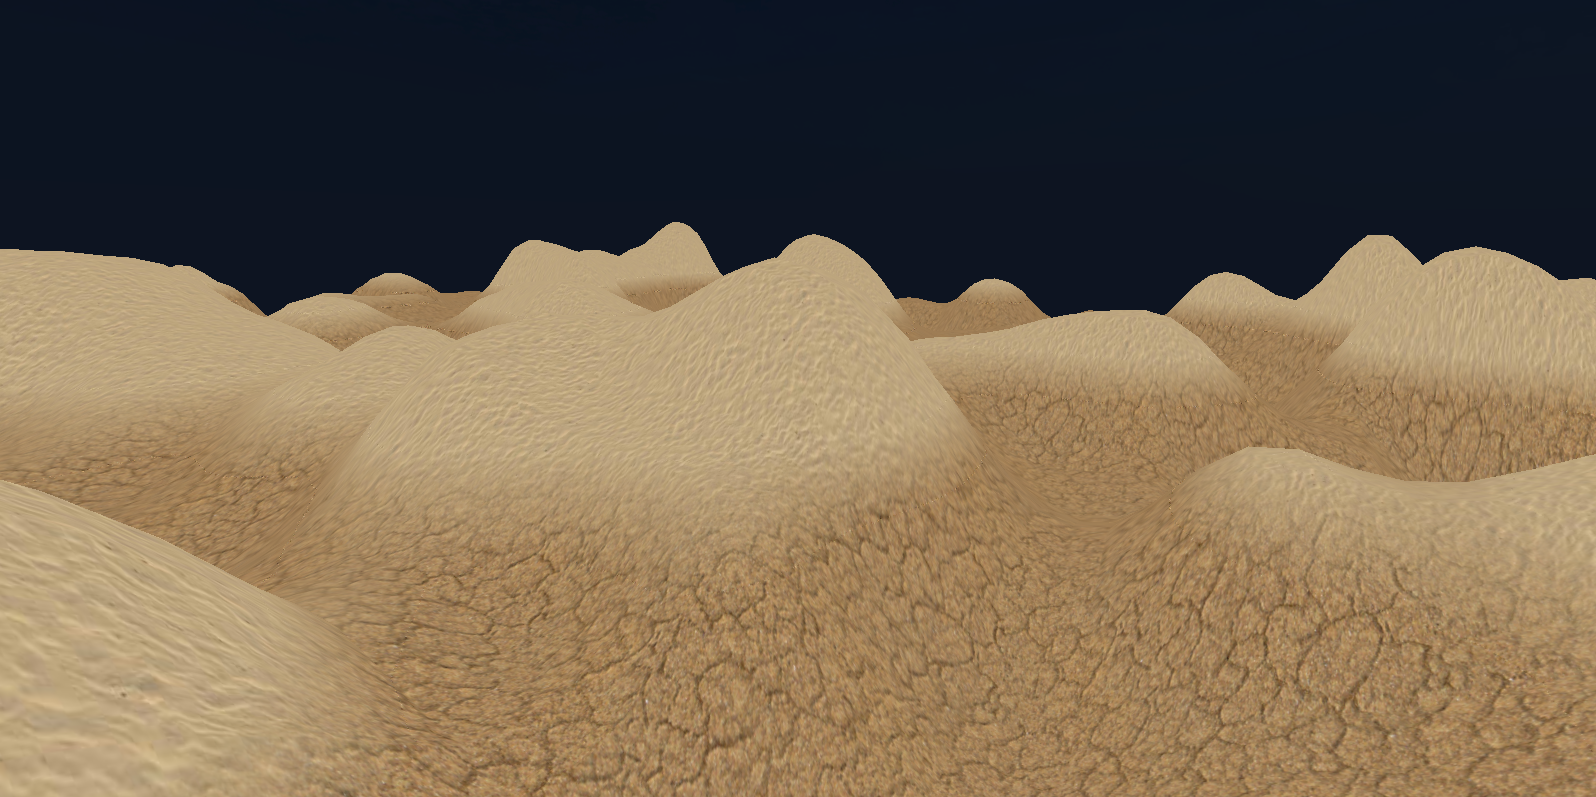
\includegraphics[width=6.3cm]{images/terrain2Texture.png} }}%
	\caption{}
\end{figure}

\subsection{References}

If you want to find the things mentioned above, you can check \textbf{terrainManagement.h}, \textbf{terrainVert.vert}, \textbf{terrainFrag.frag} files.

\newpage